\begin{tikzpicture}
\draw (-1,0) node[rectangle,draw,minimum width=.5in,minimum height=.1in] (e) {};
\draw (-1,0) node[above=9pt] {$R_{1}$};
\draw (1,0) node[rectangle,draw,minimum width=.5in,minimum height=.1in] (f) {};
\draw (1,0) node[above=9pt] {$R_{2}$};
\draw[very thick] (-2.25,0) -- (e.180);
\draw[very thick] (e.0) -- (f.180);
\draw[very thick] (f.0) -- (2.25,0);

\draw (-2,-2) node {\begin{tikzpicture}
\draw (.75,0) node[rectangle,draw,minimum width=.5in,minimum height=.1in] (e) {};
\draw[very thick] (-.5,0) -- (e.180);
\draw[very thick] (e.0) -- (2,0);
\draw (.75,0) node[above=9pt] {$R$};
\draw (-.2,.25) node[above] {$\alpha_{1}$};
\draw[<-] (-.52,0) -- node[below] {$\eta_{1}$} ++(-.5,0);
\draw[->] (2.02,0) -- node[below] {$\eta_{1}$} ++(.48,0);
\draw (1.7,.25) node[above] {$\alpha_{2}$};
\end{tikzpicture}};

\draw (2,-2) node {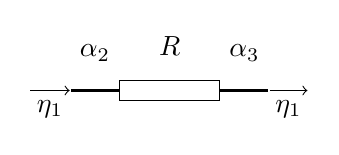
\begin{tikzpicture}
\draw (.75,0) node[rectangle,draw,minimum width=.5in,minimum height=.1in] (e) {};
\draw[very thick] (-.5,0) -- (e.180);
\draw[very thick] (e.0) -- (2,0);
\draw (.75,0) node[above=9pt] {$R$};
\draw (-.2,.25) node[above] {$\alpha_{2}$};
\draw[<-] (-.52,0) -- node[below] {$\eta_{1}$} ++(-.5,0);
\draw[->] (2.02,0) -- node[below] {$\eta_{1}$} ++(.48,0);
\draw (1.7,.25) node[above] {$\alpha_{3}$};
\end{tikzpicture}};
\end{tikzpicture}